\chapter{Teaching Your PI Controller to Behave (Part II)}

In my previous blog on this topic, we briefly reviewed the history of the PI controller and presented two forms that are commonly used today.  Regardless of which form you use, the frequency responses look identical.  But for our analysis, let’s focus on the \textit{series} form of the PI controller as shown below.

\begin{center}
    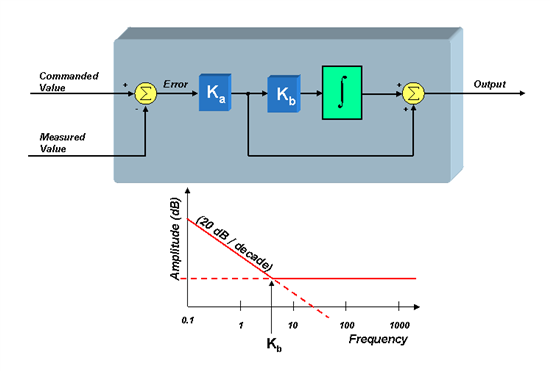
\includegraphics[width=1\linewidth]{02/01_series}
\end{center}

If you have ever done a frequency stability analysis of a control system, you probably understand why $K_a$ is so important, since it sets the gain of the PI control loop, which in turn has a pronounced effect on system stability.  But it turns out that the inflection point in the graph (the “zero” frequency) also plays a significant but perhaps more subtle role in the performance of the system.  To understand this, we will need to dive into a little math (hopefully not too much) to derive the transfer function for the PI controller, and understand how the controller’s “zero” plays a role in the overall system response.  We can define the “s-domain” transfer function from the error signal to the controller output as:
\begin{equation}
PI(s) = \frac{K_a K_b}{s} + K_a = \frac{K_aK_b \left(1+\frac{s}{K_b}\right)}{s}
\end{equation}

From this expression, we can clearly see the pole at $s = 0$, as well as the zero at $s = K_b\;(\unit{\radian\per\second})$.  So, why is the value of this zero so important?  To answer this question, let’s drop the PI controller into the heart of a current mode controller which is controlling a motor, as shown below.

\begin{center}
    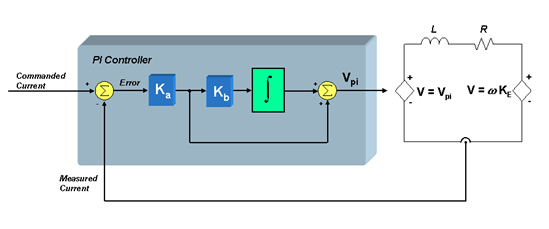
\includegraphics[width=1\linewidth]{02/02_current_mode_controller}
\end{center}

We will use a first-order approximation of the motor winding to be a simple series circuit containing a resistor, an inductor, and a back-EMF voltage source.  Assuming that the back-EMF voltage is a constant for now (since it usually changes slowly with respect to the current), we can define the small-signal transfer function from motor voltage to motor current as:
\begin{equation}
    \frac{I(s)}{V(s)} = \frac{\frac1R}{1+\frac{L}{R}s}
\end{equation}

If we also assume that the bus voltage and PWM gain scaling are included in the $K_a$ term, we can now define the “loop gain” as the product of the PI controller transfer function and the V-to-I transfer function of the RL circuit:

\begin{equation}\label{eq:3}
    G_{loop}(s) = PI(S)\cdot\frac{I(s)}{V(s)} = \left(\frac{K_aK_b \left(1+\frac{s}{K_b}\right)}{s}\right)\left(\frac{\frac1R}{1+\frac{L}{R}s}\right)
\end{equation}

To find the total system response (closed-loop gain), we must use the following expression which you probably remember from your college control systems class:

\begin{equation}\label{eq:4}
    G(s) = \frac{G_{loop}(s)}{1+G_{loop}(s)}
\end{equation}

(assuming that the feedback gain $H(s) = 1$)

Substituting \ref{eq:3} into \ref{eq:4} yields:

\begin{equation}
    G(s) = \frac{\left(\frac{K_aK_b \left(1+\frac{s}{K_b}\right)}{s}\right)\left(\frac{\frac1R}{1+\frac{L}{R}s}\right)}{1+\left(\frac{K_aK_b \left(1+\frac{s}{K_b}\right)}{s}\right)\left(\frac{\frac1R}{1+\frac{L}{R}s}\right)}
\end{equation}

I realize the expression is getting bigger instead of smaller, but don’t freak out just yet.  With a little bit of algebraic prowess, we can reduce this expression to the following:

\begin{equation}\label{eq:6}
    G(s) = \frac{\left(1+\frac{s}{K_b}\right)}{\left(\frac{L}{K_aK_b}\right)s^2 + \left(\frac{R}{K_aK_b}+\frac{1}{K_b}\right)s + 1}
\end{equation}

The denominator is a second order expression in $s$ which means there are two poles in the transfer function.  If we are not careful with how we select $K_a$ and $K_b$, we can easily end up with complex poles (Yuck!)  Depending on how close those complex poles are to the $j\omega$ axis, our system could have some really nasty resonant peaks.  So let’s assume right away that we want to select $K_a$ and $K_b$ in such a way as to avoid complex poles.  In other words, can we put the denominator in factored form so that it looks like this:

\begin{equation}\label{eq:7}
    \left(\frac{L}{K_aK_b}\right)s^2 + \left(\frac{R}{K_aK_b}+\frac{1}{K_b}\right)s + 1 = \left(1+Cs\right)\left(1+Ds\right)
\end{equation}

where $C$ and $D$ are real numbers.

If we multiply out the expression on the right side of the equation, and compare the results with the left side of the equation, we see that in order to obtain real poles, the following conditions must be satisfied:

\begin{equation}\label{eq:8}
    \frac{L}{K_aK_b} = C\cdot D
\end{equation}

and,
\begin{equation}\label{eq:9}
    \frac{R}{K_aK_b} + \frac{1}{K_b} = C + D
\end{equation}

As a first attempt to solve \ref{eq:8} and \ref{eq:9}, let’s simply equate the terms on both sides of \ref{eq:9}. In other words,

\begin{align*}
    \frac{R}{K_aK_b} &= C \\
    \frac{1}{K_b} &= D \tag{Equ. 10}\label{eq:10}
\end{align*}

The reason I recommended these substitutions will now become clear.  If we replace the denominator of \ref{eq:6} with its factored equivalent expression as shown in \ref{eq:7}, and then make the substitutions recommended in \ref{eq:10}, we get the following:

\begin{equation}\label{eq:11}
    G(s) = \frac{\left(1+\frac{s}{K_b}\right)}{\left(1+\frac{R}{K_aK_b}s\right)\left(1+\frac{s}{K_b}\right)}
\end{equation}

Notice anything interesting about this expression?  It turns out that the $D$ substitution results in a pole which cancels out the zero in the closed-loop gain expression!  By choosing $C$ and $D$ correctly, we not only end up with real poles, but we can create a closed-loop system response that has only ONE real pole and NO zeros!  No peaky frequency responses or resonant conditions!  Just a beautiful single-pole low-pass roll off response!

But wait…there’s more!  (At this point I feel like an announcer for a cheap infomercial!)  By substituting the expressions for $C$ and $D$ recommended in equation 10 back into equation 8, we get the following equality:

\begin{equation}\label{eq:12}
    K_b = \frac{R}{L}
\end{equation}

Recall that $K_b$ is the frequency at which the controller zero occurs.  So in order to get the response described in \ref{eq:11}, all we have to do is to set $K_b$ (the controller zero frequency) to be equal to the pole of the plant it is controlling!

So, now that we know how to set $K_b$, what about $K_a$?  Let’s rewrite the closed-loop system response $G(s)$, making all of the substitutions we have discussed up to now, and see what we get:

\begin{equation}\label{eq:13}
    G(s) = \frac{1}{\frac{L}{K_a}s + 1} \Rightarrow K_a= L\cdot Bandwidth \;(\unit{\radian\per\second})
\end{equation}

So we see that $K_a$ directly sets the bandwidth of the control system which is scaled by the motor’s inductance.  It turns out that numerically, $K_a$ equals the inductive impedance at whatever the bandwidth cutoff frequency is.

In summary, what have we learned?  Even if you didn’t follow all the math, there are some simple rules you can use to help you design your PI controller for your current loop:

1.  $K_b$ sets the zero of the PI controller.  When controlling a plant parameter with only one real pole in its transfer function (e.g., the current in a motor), $K_b$ should be set to the value of this pole.  Doing so will result in pole/zero cancellation, and create a closed-loop response that also only has a single real pole.  If the PI controller is part of a larger control loop, $K_b$ is not visible to the outside world since it is only used for pole-zero cancellation within the PI control loop itself.

2.  $K_a$ sets the BANDWIDTH of the closed-loop system response.  As seen by \ref{eq:13}, the higher $K_a$ is, the higher the current loop bandwidth will be.  We will discuss how to select an appropriate bandwidth in a later blog.

<Whew!>  I think I blew out enough brain cells for one blog.  I realize that this got a little “mathy,” but hopefully you could follow along with my equations.  More importantly, I hope you understand what these equations are trying to tell you about how to design your PI current control loop.  In my next blog, I want to discuss how to design a cascaded PI velocity loop which contains a PI current controller within it.  In the meantime\dots

Keep Those Motors Spinning,\\

\includegraphics[width=0.2\linewidth]{01/04_dave}
\vfill
\textit{Mar 04 2013 15:01 PM}